\documentclass[10pt,border=4pt]{standalone}
\usepackage{mathptmx}
\usepackage{amsmath,amssymb,bm}
\usepackage{tikz}
\usetikzlibrary{patterns,decorations.pathmorphing,decorations.pathreplacing,arrows.meta,fit,backgrounds,calc,positioning,shapes.geometric}
\definecolor{acc}{HTML}{0B5394}
\definecolor{accl}{HTML}{EAF0F7}
\definecolor{grp}{HTML}{F5F5F5}
\definecolor{org}{HTML}{C55A11}
\definecolor{orgl}{HTML}{FBEFE6}
\tikzset{
 dat/.style={draw=black,line width=0.6pt,fill=white,align=center,font=\small,inner sep=3pt,minimum height=0.85cm},
 lay/.style={draw=acc,line width=0.8pt,fill=accl,rounded corners=2pt,align=center,font=\small,inner sep=3pt,minimum height=0.85cm},
 cnd/.style={draw=org,line width=0.8pt,fill=orgl,rounded corners=2pt,align=center,font=\small,inner sep=3pt,minimum height=0.75cm},
 op/.style={circle,draw=black,line width=0.6pt,fill=white,inner sep=0.5pt,font=\small,minimum size=5mm},
 grpb/.style={draw=black!45,dashed,line width=0.6pt,rounded corners=3pt,inner sep=6pt},
 arr/.style={-{Latex[length=2.2mm,width=1.7mm]},line width=0.7pt},
 carr/.style={-{Latex[length=2.2mm,width=1.7mm]},line width=0.7pt,draw=org},
 shp/.style={font=\scriptsize,text=black!70,inner sep=1pt},
 lab/.style={font=\footnotesize,inner sep=1pt},
 ttl/.style={font=\small\bfseries,inner sep=0pt,anchor=west}
}
\newcommand{\xh}{\mathbf{x}_h}\newcommand{\xf}{\mathbf{x}_f}

\begin{document}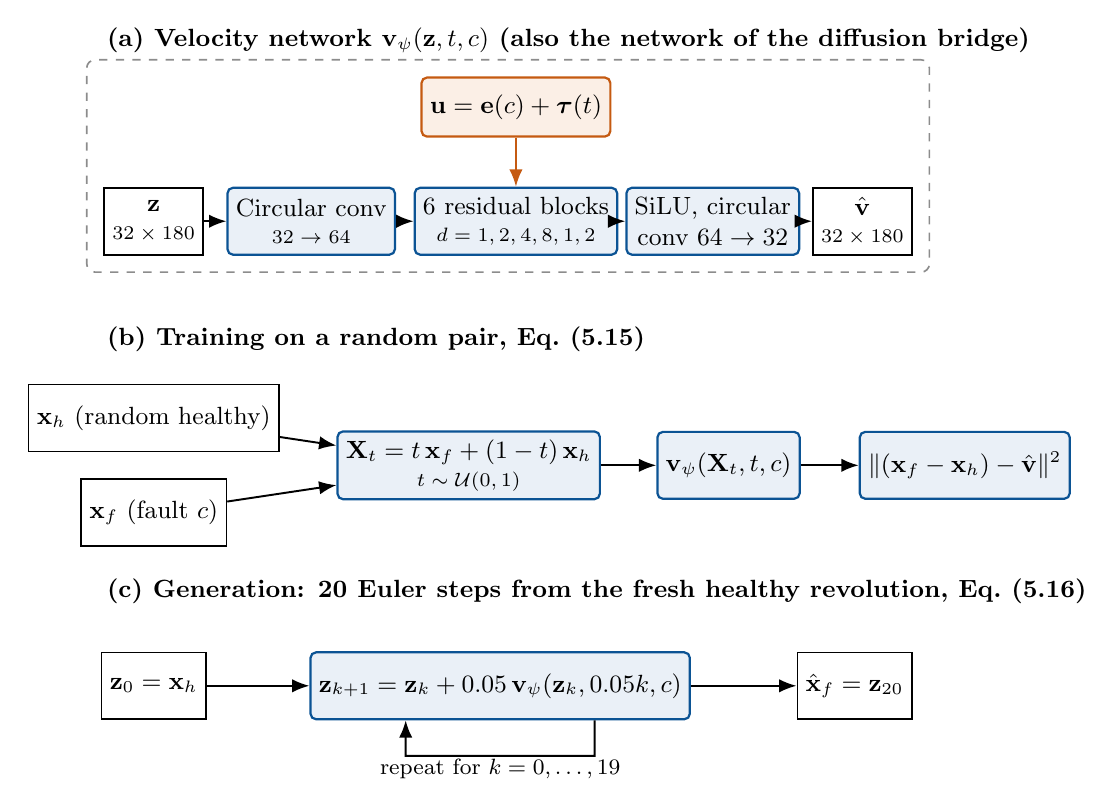
\begin{tikzpicture}[x=1cm,y=1cm]
\node[ttl] at (-0.6,2.3) {(a) Velocity network $\mathbf{v}_\psi(\mathbf{z},t,c)$ (also the network of the diffusion bridge)};
\node[dat] (z) at (0,0) {$\mathbf{z}$\\[-1pt]\scriptsize $32\times180$};
\node[lay] (s1) at (2.0,0) {Circular conv\\[-1pt]\scriptsize $32\to64$};
\node[lay] (b1) at (4.6,0) {6 residual blocks\\[-1pt]\scriptsize $d=1,2,4,8,1,2$};
\node[lay] (o1) at (7.1,0) {SiLU, circular\\conv $64\to32$};
\node[dat] (v) at (9.0,0) {$\hat{\mathbf{v}}$\\[-1pt]\scriptsize $32\times180$};
\draw[arr] (z)--(s1); \draw[arr] (s1)--(b1); \draw[arr] (b1)--(o1); \draw[arr] (o1)--(v);
\node[cnd] (u) at (4.6,1.45) {$\mathbf{u}=\mathbf{e}(c)+\boldsymbol\tau(t)$}; \draw[carr] (u)--(b1);
\begin{scope}[on background layer]\node[grpb,fit=(z)(v)(u)] {};\end{scope}
% (b) training
\node[ttl] at (-0.6,-1.5) {(b) Training on a random pair, Eq.~(5.15)};
\node[dat] (xh) at (0,-2.5) {$\xh$ (random healthy)};
\node[dat] (xf) at (0,-3.7) {$\xf$ (fault $c$)};
\node[lay] (mix) at (4.0,-3.1) {$\mathbf{X}_t=t\,\xf+(1-t)\,\xh$\\[-1pt]\scriptsize $t\sim\mathcal{U}(0,1)$};
\node[lay] (net) at (7.3,-3.1) {$\mathbf{v}_\psi(\mathbf{X}_t,t,c)$};
\node[lay] (loss) at (10.3,-3.1) {$\lVert(\xf-\xh)-\hat{\mathbf{v}}\rVert^2$};
\draw[arr] (xh)--(mix); \draw[arr] (xf)--(mix); \draw[arr] (mix)--(net); \draw[arr] (net)--(loss);
% (c) generation
\node[ttl] at (-0.6,-4.7) {(c) Generation: 20 Euler steps from the fresh healthy revolution, Eq.~(5.16)};
\node[dat] (z0) at (0,-5.9) {$\mathbf{z}_0=\xh$};
\node[lay] (st) at (4.4,-5.9) {$\mathbf{z}_{k+1}=\mathbf{z}_k+0.05\,\mathbf{v}_\psi(\mathbf{z}_k,0.05k,c)$};
\node[dat] (zo) at (8.9,-5.9) {$\hat{\mathbf{x}}_f=\mathbf{z}_{20}$};
\draw[arr] (z0)--(st); \draw[arr] (st)--(zo);
\draw[arr] ([xshift=1.2cm]st.south) -- ++(0,-0.45) -- node[lab,below]{repeat for $k=0,\dots,19$} ++(-2.4,0) -- ([xshift=-1.2cm]st.south);
\end{tikzpicture}\end{document}
